% You should title the file with a .tex extension (hw1.tex, for example)
\documentclass[11pt]{article}

\usepackage{hyperref}
\usepackage{amsmath}
\usepackage{mathtools}
\usepackage{amssymb}
\usepackage{wrapfig}
\usepackage{fancyhdr}
\usepackage{tikz-qtree}
\usepackage{tikz-qtree-compat}
\usepackage[normalem]{ulem}
\usepackage{tikz}
\usepackage{systeme}
\usepackage{graphicx}
\DeclareMathOperator*{\argmin}{argmin}
\DeclareMathOperator*{\argmax}{argmax}
\usepackage{bm}

\oddsidemargin0cm
\topmargin-2cm     %I recommend adding these three lines to increase the 
\textwidth16.5cm   %amount of usable space on the page (and save trees)
\textheight23.5cm  

\newcommand{\question}[2] {\vspace{.25in} \hrule\vspace{0.5em}
\noindent{\bf #1: #2} \vspace{0.5em}
\hrule \vspace{.10in}}
\renewcommand{\part}[1] {\vspace{.10in} {\bf (#1)}}

\newcommand{\myname}{Sean Bittner}
\newcommand{\myandrew}{srb2201@columbia.edu}
\newcommand{\myhwnum}{12}

\setlength{\parindent}{0pt}
\setlength{\parskip}{5pt plus 1pt}
 
\DeclarePairedDelimiter\abs{\lvert}{\rvert}%
 %
\pagestyle{fancyplain}
\rhead{\fancyplain{}{\myname\\ \myandrew}}

\begin{document}

\medskip                        % Skip a "medium" amount of space
                                % (latex determines what medium is)
                                % Also try: \bigskip, \littleskip

\thispagestyle{plain}
\begin{center}                  % Center the following lines
{\Large Draft of new SC section} \\
Sean Bittner and Alex Piet \\
December 11, 2020 \\
\end{center}

\section{Identifying neural mechanisms of flexible task switching} \label{results_SC}
In a rapid task switching experiment \cite{duan2015requirement}, rats were explicitly cued on each trial to either orient towards a visual stimulus in the Pro (P) task or orient away from a visual stimulus in the Anti (A) task (Fig. \ref{fig:SC}A). 
Neural recordings in the midbrain superior colliculus (SC) exhibited two populations of neurons that simultaneously represented both task context (Pro or Anti) and motor response (contralateral or ipsilateral to the recorded side): the Pro/Contra and Anti/Ipsi neurons \cite{duan2018collicular}.
Duan et al. proposed a model of SC that, like the V1 model analyzed in the previous section, is a four-population dynamical system.  
We analyzed this model, where the neuron-type populations are functionally-defined as the Pro- and Anti-populations in each hemisphere (left (L) and right (R)), their connectivity is parameterized geometrically  (Fig. \ref{fig:SC}B).
The input-output function of this model is chosen such that the population responses $\mathbf{x} = [x_{LP}, x_{LA}, x_{RP}, x_{RA}]^\top$ are bounded from 0 to 1 as a function $f$ of a dynamically evolving internal variable $\mathbf{u}$.
The dynamics evolve with timescale $\tau=0.09$ governed by connectivity weights $W$
\begin{equation}
\begin{split}
\tau \frac{d\mathbf{u}}{dt} &= -\mathbf{u} + W\mathbf{x} + \mathbf{h} + d\mathbf{B} \\
\mathbf{x} &= f(\mathbf{u})
\end{split}
\end{equation}
with white noise of variance $\epsilon^2 = 0.2^2$.
The input $\mathbf{h}$ is comprised of a cue-dependent input to the Pro or Anti populations, a stimulus orientation input to either the Left or Right populations, and a choice-period input to the entire network (see Section \ref{methods_SC}).
Here, we use EPI to determine the changes in network connectivity $\mathbf{z} = [sW, vW, dW, hW]^{\top}$ resulting in execution of rapid task switching behavior.

\begin{figure}
\begin{center}
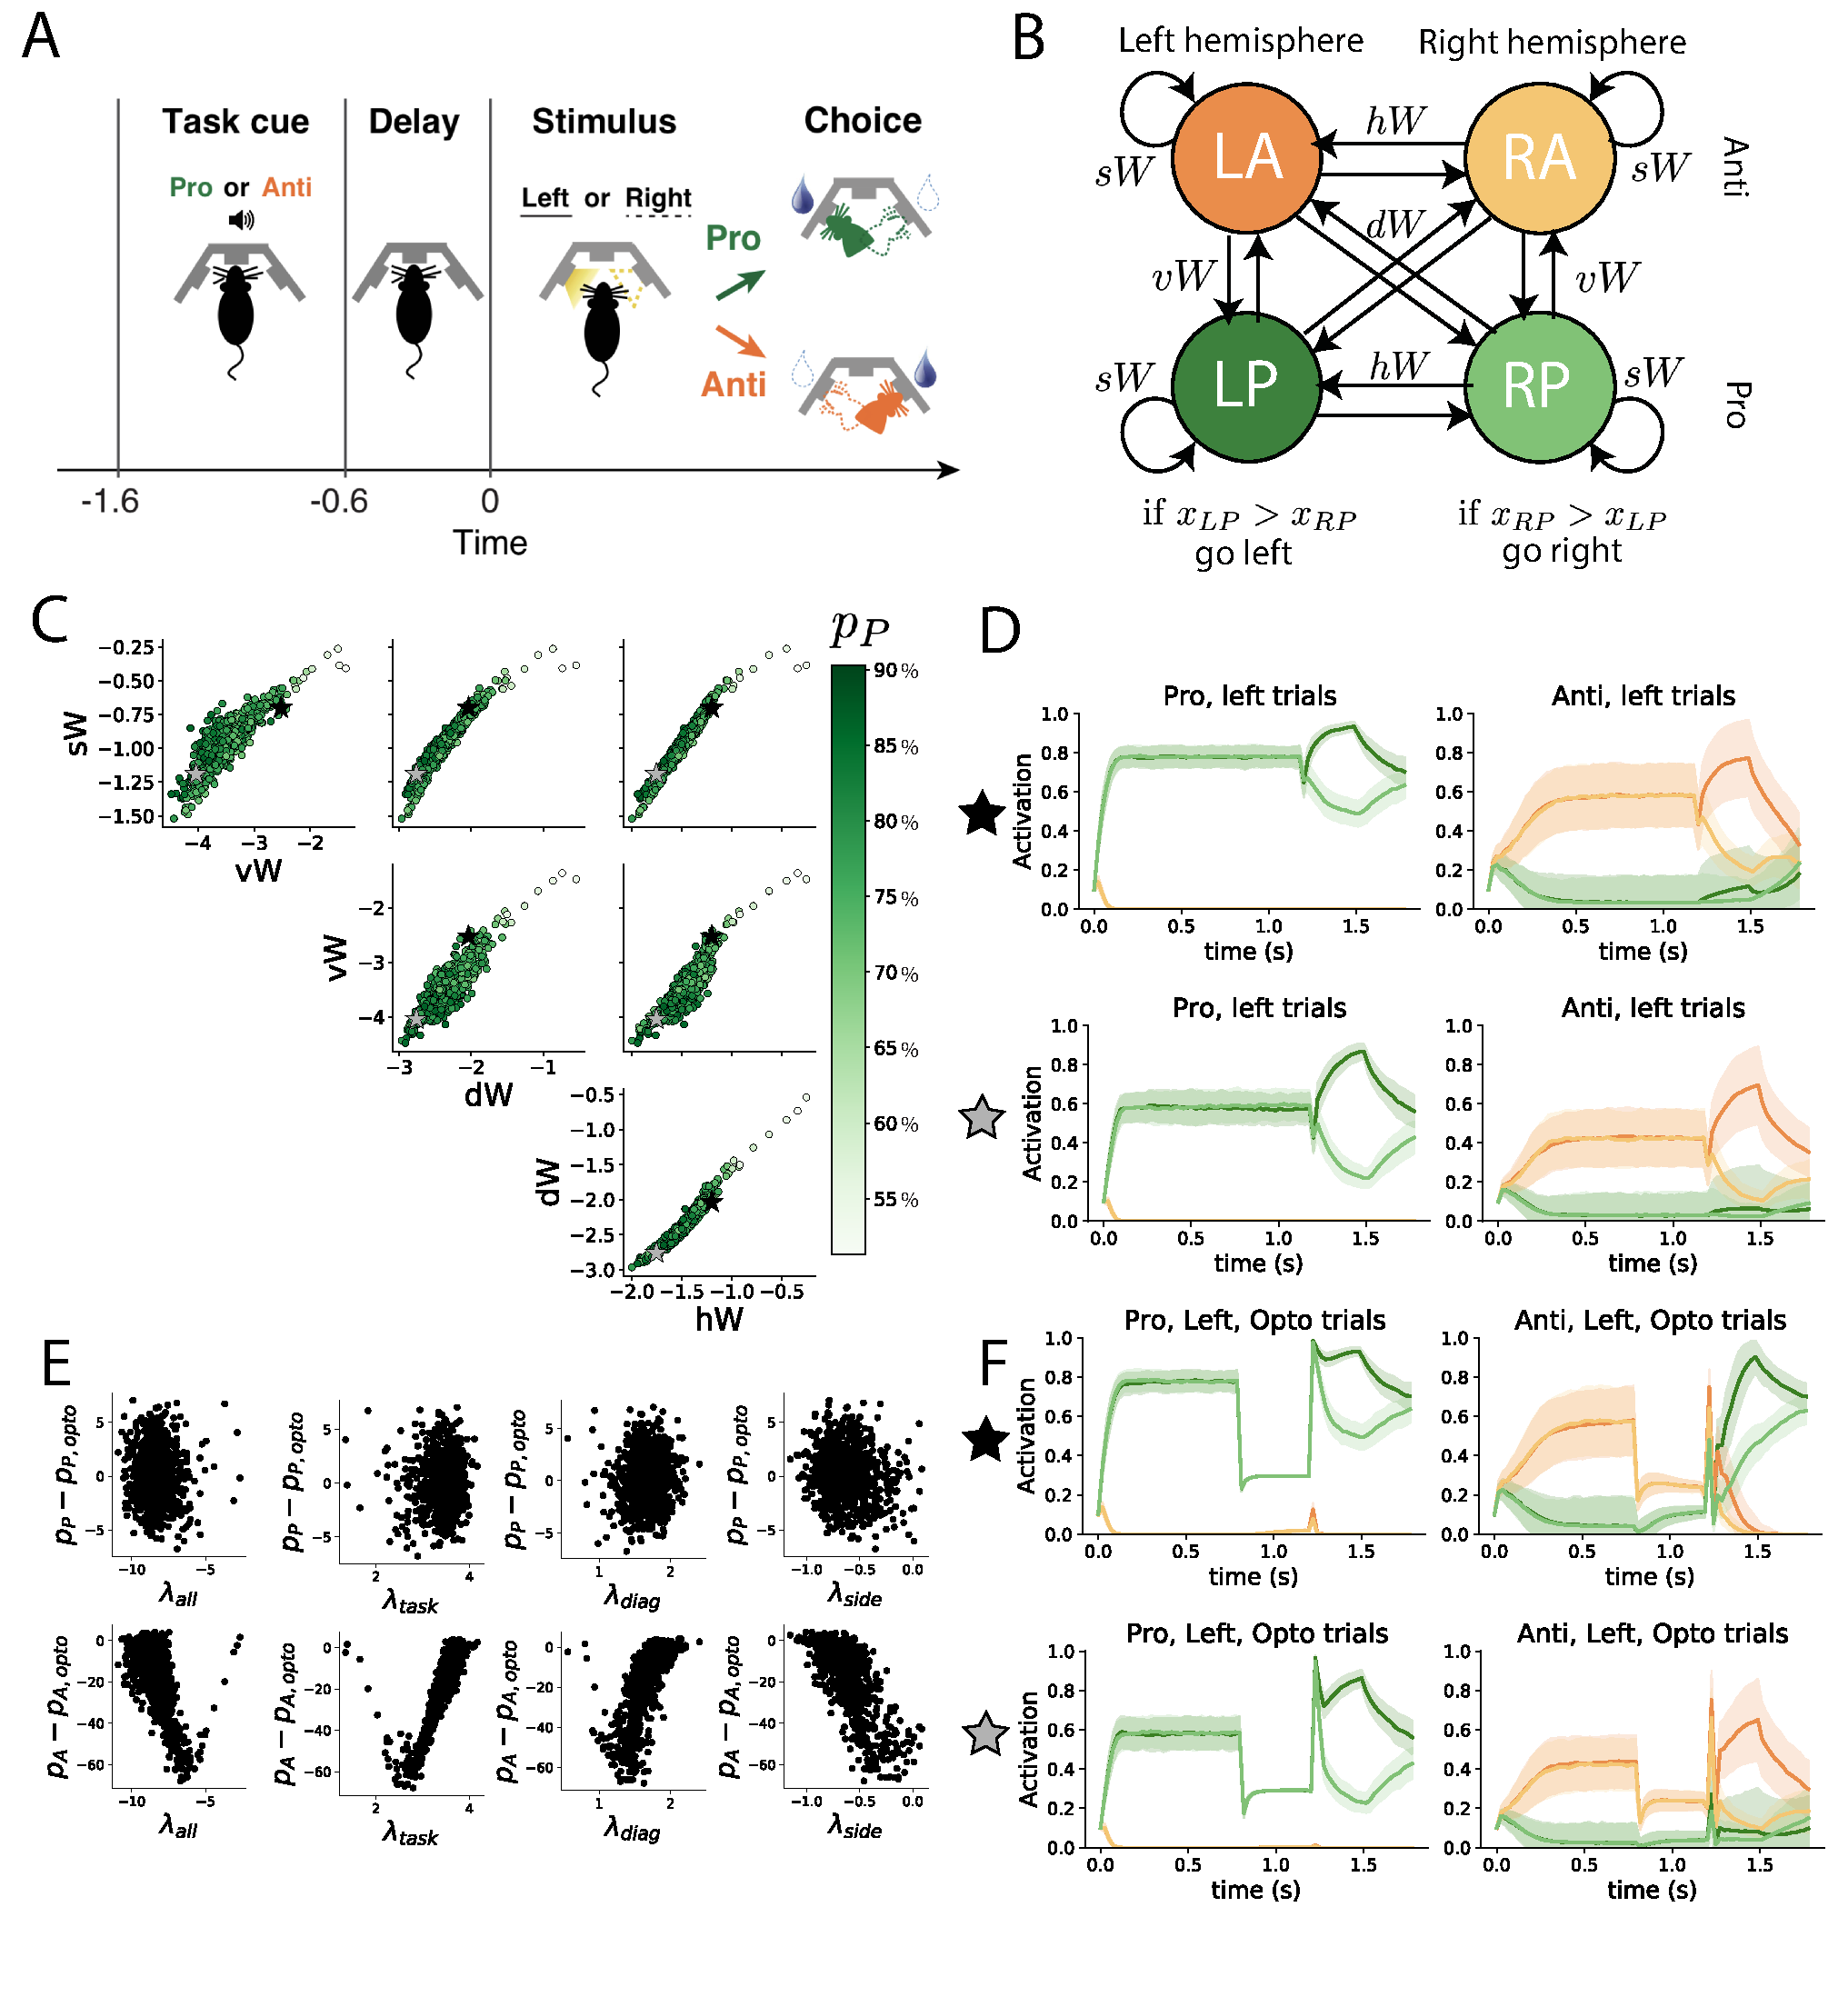
\includegraphics[scale=0.48]{figs/fig4.pdf}
\end{center}
\caption{\small 
A. Rapid task switching behavioral paradigm (see text). 
B. Model of superior colliculus (SC). Neurons: LP - left pro, RP - right pro, LA - left anti, RA - right anti. 
Parameters: $sW$ - self, $hW$ - horizontal, $vW$ -vertical, $dW$ - diagonal weights.  
Subscripts $P$ and $A$ of connectivity weights indicate Pro or Anti populations.
C. The EPI parameter distribution of rapid task switching networks.  Black star indicates parameter choice u=of simulations.
D. Simulations of an SC network from the EPI distribution with 75\% accuracy in each task.  Top row shows no inactivation during Pro and Anti trials, and bottom row shows simulations with delay period inactivation (opto strength 0.7).  Shading indicates standard deviation across trials.
E. The effect of delay period inactivation on accuracy versus dynamics eigenvalues.
}
\label{fig:SC}
\end{figure}

We define rapid task switching behavior as accurate execution of each task.  Inferred models should not exhibit fully random responses (50\%), or perfect performance (100\%), since perfection is never attained by even the best trained rats.
We formulate rapid task switching as an emergent property by stipulating that the average accuracy in the Pro task $p_P(\mathbf{x}, \mathbf{z})$ and Anti task $p_A(\mathbf{x}, \mathbf{z})$ be $75\%$ with variance $5\%^2$.
\begin{equation}\label{eq:EP}
\begin{split}
\mathcal{X} ~~:~~ \mathbb{E}_{\mathbf{z}}\begin{bmatrix} p_P(\mathbf{x}; \mathbf{z}) \\ p_A(\mathbf{x}; \mathbf{z}) \end{bmatrix}  &~~=~~  \begin{bmatrix} 75\% \\ 75\% \end{bmatrix}  \\ 
 \text{Var}_{\mathbf{z}}\begin{bmatrix} p_P(\mathbf{x}; \mathbf{z}) \\ p_A(\mathbf{x}; \mathbf{z}) \end{bmatrix}  &~~=~~  \begin{bmatrix} 5\%^2 \\ 5\%^2  \end{bmatrix}
\end{split}
\end{equation}
A variance of $5\%$ performance in each task will confer a posterior producing performances ranging from about $65\%-85\%$, allowing us to examine the properties of connectivity that yield better performance.

We ran EPI to obtain SC model connectivity parameters $z$ producing rapid task switching (Fig. \ref{fig:SC}C, Fig. \ref{fig:SX5}).
Each parameter is predictive of accuracy in either task (Fig. \ref{fig:SX1}), and may have the same ($vW$ and $dW$) or opposite ($sW$ and $hW$) effects on $p_P$ and $p_A$.
To make sense of this inferred distribution, we took the eigendecomposition of the symmetric connectivity matrices $W = V\Lambda V^{-1}$, which results in the same basis vectors $v_i$ for all $W$ parameterized by $z$ (Fig. \ref{fig:SX2}A). 
These basis vectors have intuitive roles in processing for this task, and are accordingly named the \textit{all} mode - all neurons co-fluctuate, \textit{side} mode - one side dominates the other, \textit{task} mode - the Pro or Anti populations dominate the other, and \textit{diag} mode - Pro- and Anti-populations of opposite hemispheres dominate the opposite pair. 

Smaller $\lambda_{\text{all}}$ and greater $\lambda_{\text{side}}$ predict greater accuracy in both tasks (Fig. \ref{fig:SX2}B) suggesting that wide separation between Left and Right populations at the end of stimulus presentation and fast decaying dynamics during the choice period yield better performance in both tasks.
Since the Pro neurons receive a positive bias input $h_{P, bias}$, $\lambda_{\text{task}}$ is not as important to performance in the Pro task as in the Anti task (Fig. \ref{fig:SX2}B).
The diagonal mode, hypothesized to be crucial for processing in the Anti task, was ultimately anticorrelated with $p_A$, 
This suggests that $p_A$ increases with dynamics having stronger task and stimulus representations and faster decaying dynamics in alternate dimensions.

In agreement with experimental results form Duan et al., we found that inactivation above nominal strength during the delay period consistently decreased performance in the Anti task, but had no consistent effect on the Pro task (Fig. \ref{fig:SX3}), e.g. (Fig. \ref{fig:SC}D, bottom).
Interestingly, the trends in eigenvalues that result in greater $p_A$ increase the error from delay period inactivation in the Anti task ($p_A - p_{A, opto}$) (Fig. \ref{fig:SC}E.
Despite these opposing effects, $p_A$ is uncorrelated with ($p_A - p_{A, opto}$), while $p_P$ is correlated (Fig. \ref{fig:SX4}).
This shows that the degree of error introduced by delay period inactivation is controlled by the dynamical mechanisms controlling success in the Pro task (namely $\lambda_{\text{task}}$ and $\lambda_{\text{side}}$).
Such comparable dynamics between the non-inactivated Pro task and the delay period inactivated Anti task are salient in simulations (Fig. \ref{fig:SC}D top-left and bottom-right).



\section{Supplementary}\label{methods_SC}
\begin{equation}
\mathbf{x}_\alpha = f(\mathbf{u}) = \left(\frac{1}{2}\tanh\left(\frac{u_\alpha - \epsilon}{\zeta}\right)+ \frac{1}{2} \right)
\end{equation}
where $\epsilon = 0.05$ and $\zeta = 0.5$.  

The accuracies of $p_P$ and $p_A$ are calculated as
\begin{equation}
p_P(\mathbf{x}; \mathbf{z}) = \mathbb{E}_{\mathbf{x} \sim p(\mathbf{x} \mid \mathbf{z})}\left[\Theta[x_{LP}(t=1.8s) - x_{RP}(t=1.8s)]\right]
\end{equation}
and 
\begin{equation}
p_A(\mathbf{x}; \mathbf{z}) = \mathbb{E}_{\mathbf{x} \sim p(\mathbf{x} \mid \mathbf{z})}\left[\Theta[x_{RP}(t=1.8s) - x_{LP}(t=1.8s)]\right]
\end{equation}
given that the stimulus is on the left side, where $\Theta$ is the Heaviside step function.

The Heaviside step function is approximated as
\begin{equation}
\Theta(\mathbf{x}) = \text{sigmoid}(\beta \mathbf{x}),
\end{equation}
where $\beta = 100$.

The system receives five inputs throughout each trial, which has a total length of 1.8s.
\begin{equation}
\mathbf{h}(t) = \mathbf{h}_{\text{constant}} + \mathbf{h}_{\text{P,bias}} + \mathbf{h}_{\text{rule}}(t) + \mathbf{h}_{\text{choice-period}}(t) + \mathbf{h}_{\text{light}}(t).
\end{equation}

There are rule-based inputs depending on the condition,
\begin{equation} 
\mathbf{h}_{\text{constant}} = I_{\text{constant}} [1, 1, 1, 1]^\top
\end{equation}
\begin{equation} 
\mathbf{h}_{\text{P,bias}} = I_{\text{P,bias}} [1, 0, 1, 0]^\top
\end{equation}
\begin{equation} \mathbf{h}_{\text{P,rule}}(t) = \begin{cases}
                           I_{\text{P,rule}} [1, 0, 1, 0]^\top,& \text{if } t\leq 1.2s \\
                            0,              & \text{otherwise}
                         \end{cases}
\end{equation}
\begin{equation} \mathbf{h}_{\text{A,rule}}(t) = \begin{cases}
                           I_{\text{A,rule}} [0, 1, 0, 1]^\top,& \text{if } t\leq 1.2s \\
                            0,              & \text{otherwise}
                         \end{cases}
\end{equation}
a choice-period input,
\begin{equation} \mathbf{h}_{\text{choice}}(t) = \begin{cases}
                           I_{\text{choice}} [1, 1, 1, 1]^\top,& \text{if } t > 1.2s \\
                            0,              & \text{otherwise}
                         \end{cases}
\end{equation}
and an input to the right or left-side depending on where the light stimulus is delivered.     
\begin{equation}  \mathbf{h}_{\text{light}}(t) = \begin{cases}
                           I_{\text{light}} [1, 1, 0, 0]^\top,& \text{if } t > 1.2s \text{ and Left} \\
                           I_{\text{light}} [0, 0, 1, 1]^\top,& \text{if } t > 1.2s \text{ and Right} \\
                            0,              & t \leq 1.2s
                         \end{cases} .
\end{equation}
The input parameterization was fixed to $I_{\text{constant}} = 0.75$, $I_{\text{P,bias}} = 0.5 $, $I_{\text{P,rule}} = 0.6$,  $I_{\text{A,rule}} = 0.6$,  $I_{\text{choice}} = 0.25$,  and $I_{\text{light}} = 0.5$.

\begin{figure}
\begin{center}
\includegraphics[scale=0.6]{figs/figSX5.pdf}
\end{center}
\caption{\small The EPI parameter distribution of Fig. 1C with reference to a unity line.
}
\label{fig:SX5}
\end{figure}

\begin{figure}
\begin{center}
\includegraphics[scale=0.85]{figs/figSX1.pdf}
\end{center}
\caption{\small Connectivity parameters of EPI distributions versus task accuracies.  $\beta$ is slope coefficient of linear regression, $r$ is correlation, and $p$ is the two-tailed p value.
}
\label{fig:SX1}
\end{figure}

\begin{figure}
\begin{center}
\includegraphics[scale=1.3]{figs/figSX2.pdf}
\end{center}
\caption{\small 
A. Invariant eigenvectors of connectivity matrix $W$.
B. Eigenvalues of connectivities of EPI distribution versus task accuracies.}
\label{fig:SX2}
\end{figure}

\begin{figure}
\begin{center}
\includegraphics[scale=0.6]{figs/figSX4.pdf}
\end{center}
\caption{\small 
Difference in performance of each task during inactivation.  Inactivation level ``opto strength" scales from no inactivation (0) to full inactivation (1).  We compare delay period inactivation $1.2 < t < 1.5$ (blue), choice period inactivation $1.5 < t$ (red), and total inactivation $0 \leq t \leq 1.8$ (purple).
}
\label{fig:SX3}
\end{figure}

\begin{figure}
\begin{center}
\includegraphics[scale=0.75]{figs/figSX3.pdf}
\end{center}
\caption{\small Scatters of the effect of delay period inactivation in each task with task accuracy.  Plots are shown at an opto strength of 0.7.
}
\label{fig:SX4}
\end{figure}

%
%\begin{figure}
%\begin{center}
%\includegraphics[scale=0.6]{figs/figSX2.pdf}
%\end{center}
%\caption{\small
%Same as Fig. 1C shaded by Anti task accuracy.}
%\label{fig:SC_EPI2}
%\end{figure}


\bibliography{epi}
\bibliographystyle{unsrt}

\end{document}